% pipeline — hand-authored TikZ figure (absolute coordinates; no auto-layout).
% Build:  bash docs/figures/build.sh pipeline
% Palette, box shapes and arrow idioms are shared with retrieval.tex, which zooms into the
% "Search" box drawn here; a change to either belongs in both.
%
% The drawing is an INSIGHT INTO THE METHOD, not a specification, and it sits at the top of a
% README with no caption under it. So: node titles are one or two words, an italic sub-label
% survives only where a reader would otherwise misread the box, and an edge carries a label only
% when the arrow alone would be read wrongly. The \parbox caption below is for the paper and
% carries every explanation the drawing deliberately drops.
\documentclass[border=8pt,varwidth=210mm]{standalone}
\usepackage{tikz}
\usetikzlibrary{shapes.geometric,arrows.meta,calc,backgrounds}

\definecolor{bluevar}{HTML}{2F6BC0}
\definecolor{ambervar}{HTML}{C5701F}
\definecolor{greenvar}{HTML}{1B7A3E}
\definecolor{slatefill}{HTML}{E9EDF2}
\definecolor{slatestroke}{HTML}{4A5563}
\definecolor{modstroke}{HTML}{33404F}
\definecolor{loopstroke}{HTML}{555F6B}

% Caption switch, same name and default in both figure sources. The caption is drawn inside the
% exported image, and the README already carries that text in its prose, so it is off unless the
% build defines \withcaption: CAPTION=1 bash docs/figures/build.sh pipeline.
\newif\ifshowcaption
\showcaptionfalse
\ifdefined\withcaption\showcaptiontrue\fi

\begin{document}
\centering
% No hyphenation inside the drawing: a box label broken as "of the cor-pus" reads as a typo, and
% every label here is short enough to wrap on a word. The group keeps this local to the picture,
% so the caption below still hyphenates normally. Same treatment as the companion figure.
{\hyphenpenalty=10000 \exhyphenpenalty=10000 \tolerance=9999 \emergencystretch=2em
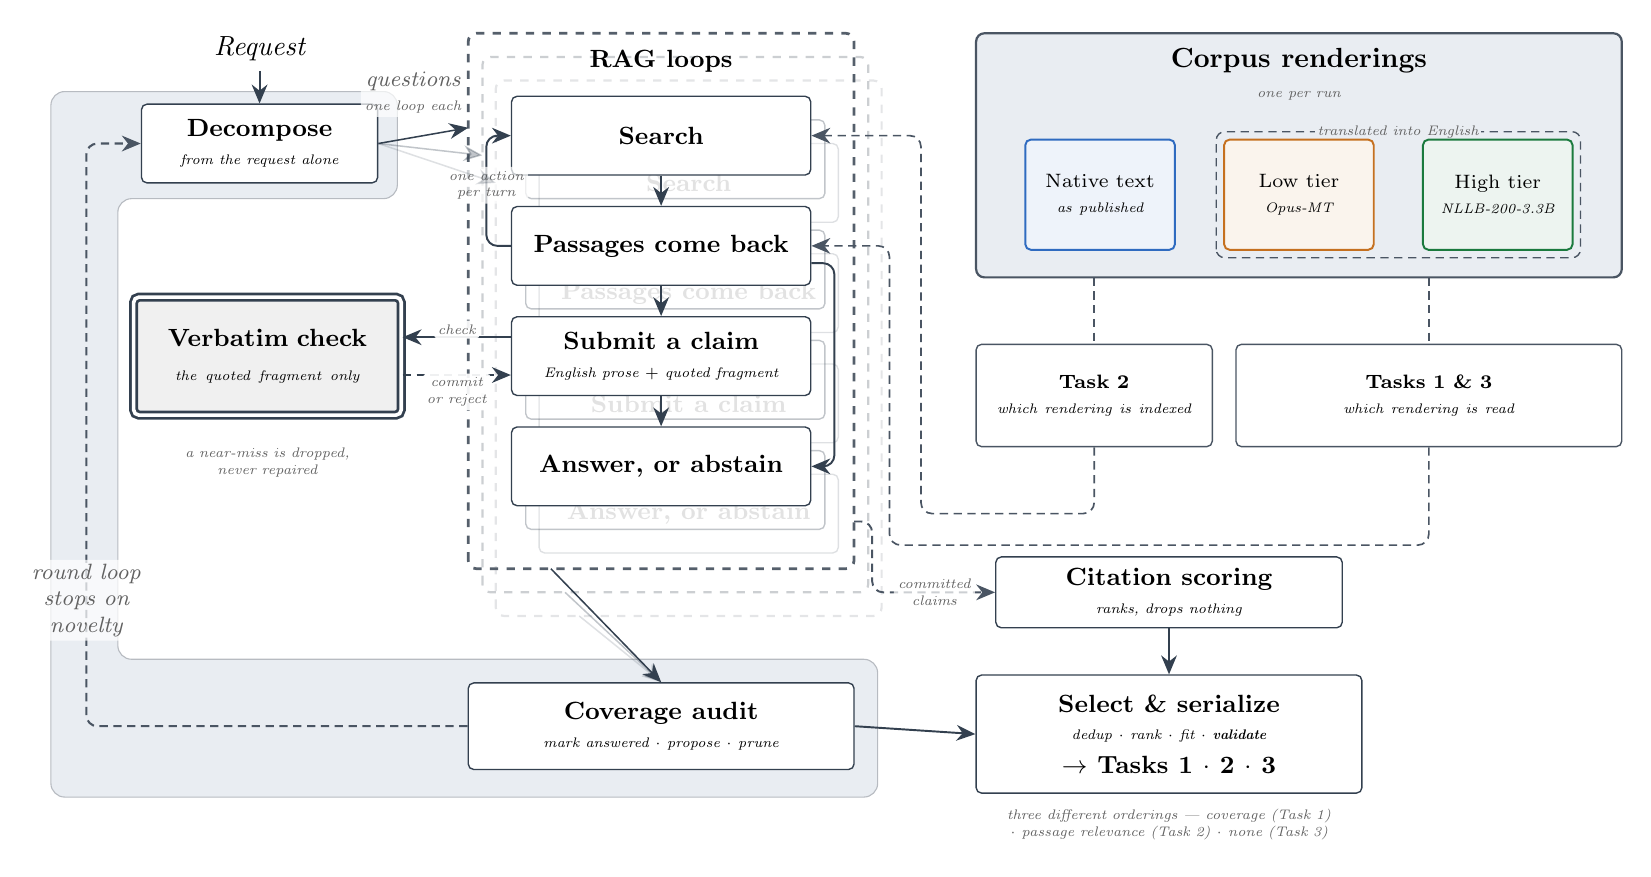
\begin{tikzpicture}[
  >={Stealth[length=2.4mm,width=2mm]},
  font=\small,
  mod/.style={draw=modstroke,line width=0.5pt,fill=white,rounded corners=2pt,
              align=center,minimum width=38mm,minimum height=10mm,inner sep=2pt},
  flow/.style={draw=modstroke,line width=0.7pt,->},
  fan/.style={draw=modstroke,line width=0.55pt,->},
  runedge/.style={draw=slatestroke,line width=0.6pt,->,densely dashed},
  comp/.style={align=center,text width=17mm,draw,line width=0.7pt,
               minimum width=19mm,minimum height=14mm,inner sep=1pt,font=\scriptsize},
  taskbox/.style={align=center,text width=21mm,draw=slatestroke,line width=0.5pt,fill=white,
                  rounded corners=2pt,minimum width=25.3mm,minimum height=13mm,inner sep=2pt,
                  font=\scriptsize},
  note/.style={font=\tiny\itshape,text=black!62,align=center},
  % white backing so a label stays legible over an arrow; font in OPTIONS (not inline) so the
  % WHOLE multi-line label is styled, not just its first line:
  lbl/.style={fill=white,fill opacity=0.72,text opacity=1,inner sep=1.5pt,rounded corners=1.5pt,
              font=\footnotesize\itshape,text=black!62,align=center},
]

% ---------- helper: loop CONTENT for the FADED piled copies (modules only, NO title) ----------
\newcommand{\loopcontent}[3]{% #1=dx  #2=dy  #3=opacity
  \begin{scope}[shift={(#1,#2)},opacity=#3]
    \draw[dashed,draw=loopstroke,line width=0.8pt,rounded corners=3pt] (4.55,5.0) rectangle (9.45,11.8);
    \node[mod] at (7,10.5){\bfseries Search};
    \node[mod] at (7,9.1) {\bfseries Passages come back};
    \node[mod] at (7,7.7) {\bfseries Submit a claim};
    \node[mod] at (7,6.3) {\bfseries Answer, or abstain};
  \end{scope}}

% ---------- faded piled copies BEHIND (drawn first); near copy = (0.18,-0.30), far = (0.35,-0.60) ----
\loopcontent{0.35}{-0.60}{0.16}
\loopcontent{0.18}{-0.30}{0.30}

% ===== SHARED MODULE ENCLOSURE: Decompose + Coverage audit, iterated by round =====
% Subtle L-shaped backing (background layer) that hugs the round loop: it wraps Decompose
% (top-left, round 0), runs down the far-left riser (the round-loop back-edge), and wraps
% Coverage audit (bottom, later rounds). Concave on purpose, so it does not cover the
% RAG-loops / verbatim-check / citation-scoring boxes that live in the (white) centre. Tint =
% slatefill (the same light grey as the corpus grouping box) so it reads as "one grouped unit".
\begin{scope}[on background layer]
  \fill[slatefill,rounded corners=5pt]
     (-0.75,11.06) -- (3.65,11.06) -- (3.65,9.70) -- (0.10,9.70) --
     (0.10,3.85) -- (9.75,3.85) -- (9.75,2.10) -- (-0.75,2.10) -- cycle;
  \draw[slatestroke!40,line width=0.4pt,rounded corners=5pt]
     (-0.75,11.06) -- (3.65,11.06) -- (3.65,9.70) -- (0.10,9.70) --
     (0.10,3.85) -- (9.75,3.85) -- (9.75,2.10) -- (-0.75,2.10) -- cycle;
\end{scope}

% ================= REQUEST (text) -> DECOMPOSE  (TOP-LEFT corner) =================
\node[align=center,font=\itshape] (request) at (1.9,11.6) {Request};
% The ONE sub-label that survives here: round 0 sees no evidence, which the arrows cannot show.
\node[mod,minimum width=30mm] (decompose) at (1.9,10.4)
   {{\bfseries Decompose}\\[-1pt]{\tiny\itshape from the request alone}};
\draw[flow] (request) -- (decompose);

% ================= RAG LOOPS (front, full opacity — the ONLY title) =================
\draw[dashed,draw=loopstroke,line width=1pt,rounded corners=3pt] (4.55,5.0) rectangle (9.45,11.8);
\node at (7,11.45) {\bfseries RAG loops};
\node[mod] (retrieval) at (7,10.5) {\bfseries Search};
\node[mod] (read)      at (7,9.1)  {\bfseries Passages come back};
% The one thing a reader gets backwards here: what commits is not the quote.
\node[mod] (claim)     at (7,7.7)
   {{\bfseries Submit a claim}\\[-1pt]{\tiny\itshape English prose $+$ quoted fragment}};
% STOPPING SCOPE 1 of 2 (per question); the round-loop scope is labelled on the back-edge.
% "abstain" carries the termination on its own, so this box needs no sub-label.
\node[mod] (answer)    at (7,6.3) {\bfseries Answer, or abstain};

% A search really does cause the passages to come back, so that edge stays solid. The two below
% it are choices, not steps: the bypass shows that the model may close straight from the passages.
\draw[flow] (retrieval) -- (read);
\draw[flow] (read) -- (claim);
\draw[flow] (claim) -- (answer);
\draw[flow,rounded corners=4pt]
   ([yshift=-2.2mm]read.east) -- (9.2,8.88) -- (9.2,6.3) -- (answer.east);
% agentic recurrence: the WHOLE menu is re-offered every turn, not just the searching step.
% Routed read.west (y=9.1) -> search.west (y=10.5) so it clears the commit box arrows at y=7.7.
\draw[flow,rounded corners=4pt] (read.west) -- (4.78,9.1) --
   node[lbl,pos=0.55,font=\tiny\itshape]{one action\\per turn} (4.78,10.5) -- (retrieval.west);

% Decompose --(one-to-many fan)--> each of the THREE pile layers (front/near/far left edges)
\node[lbl] at (3.85,11.05) {questions\\[-1pt]{\tiny one loop each}};
% only the FRONT-layer arrow is opaque; the other two are as faded as the layer they hit.
\draw[fan] (decompose.east) -- (4.55,10.6);
\draw[fan,opacity=0.30] (decompose.east) -- (4.73,10.25);
\draw[fan,opacity=0.16] (decompose.east) -- (4.90,9.90);

% ================= COVERAGE AUDIT (below the RAG loops; the OUTER coverage loop) ==============
% Same mod style; sits AFTER the loops. Width matches the loop container (4.9cm). The fan arrows
% below already say "it reads what the loops found", so that clause is not repeated in words.
\node[mod,minimum width=49mm,minimum height=11mm] (audit) at (7,3.0)
   {{\bfseries Coverage audit}\\[-1pt]{\tiny\itshape mark answered $\cdot$ propose $\cdot$ prune}};
% many-to-one fan FROM the three pile layers: exact mirror of the decompose fan -- three distinct
% sources on the loop's bottom (the three pile layers), all converging to ONE single point
% (audit.north, the top-centre). Opacity graded to match the layer each source belongs to.
\draw[fan] (5.6,5.0) -- (audit.north);
\draw[fan,opacity=0.30] (5.78,4.70) -- (audit.north);
\draw[fan,opacity=0.16] (5.96,4.40) -- (audit.north);

% ================= SELECT & SERIALIZE — TERMINAL box, to the RIGHT of the audit, SAME y-level ====
\node[mod,minimum width=49mm,minimum height=15mm] (report) at (13.45,2.9)
   {{\bfseries Select \& serialize}\\[-1pt]{\tiny\itshape dedup $\cdot$ rank $\cdot$ fit $\cdot$ \textbf{validate}}\\[1pt]{\bfseries $\to$ Tasks~1 $\cdot$ 2 $\cdot$ 3}};
% Coverage audit -> Select & serialize: short straight HORIZONTAL arrow into the terminal.
\draw[flow] (audit.east) -- (report.west);
% "rank" is the word doing the most hiding: there is no single ranking, there are three.
\node[note,text width=56mm] at (13.45,1.75)
   {three different orderings --- coverage (Task~1) $\cdot$ passage relevance (Task~2) $\cdot$ none (Task~3)};

% ================= CORPUS RENDERING BOX (TOP-RIGHT corner) =================
\begin{scope}[on background layer]
  \fill[slatefill,rounded corners=3pt] (11.0,8.7) rectangle (19.2,11.8);
  \draw[slatestroke,line width=0.8pt,rounded corners=3pt] (11.0,8.7) rectangle (19.2,11.8);
\end{scope}
\node[font=\bfseries] at (15.1,11.45) {Corpus renderings};
\node[note] at (15.1,11.0) {one per run};
% Three EQUAL chips EVENLY spaced (outer margin = inner gap = 0.625): centres 12.575 / 15.1 /
% 17.625, all at y=9.75. Order is native, then the WEAKER translation, then the stronger one, so
% the row ascends left to right. Colour travels WITH the tier, never with the position: blue is
% "no translation", amber is the low tier, green is the high tier, here and in the companion
% figure's caption. Native stands alone; the two translation tiers are framed by the sub-box,
% whose borders sit centred in the native->low-tier gap and the right margin so the spacing
% still reads even.
\node[comp,rounded corners=2pt,draw=bluevar,fill=bluevar!8]
      at (12.575,9.75) {Native text\\[1pt]{\tiny\itshape as published}};
\draw[slatestroke,line width=0.5pt,densely dashed,rounded corners=3pt]
      (14.05,8.95) rectangle (18.675,10.55);
\node[font=\tiny\itshape,text=black!62,fill=slatefill,inner sep=1pt] at (16.36,10.55)
      {translated into English};
\node[comp,rounded corners=2pt,draw=ambervar,fill=ambervar!8]
      at (15.1,9.75) {Low tier\\[1pt]{\tiny\itshape Opus-MT}};
\node[comp,rounded corners=2pt,draw=greenvar,fill=greenvar!8]
      at (17.625,9.75) {High tier\\[1pt]{\tiny\itshape NLLB-200-3.3B}};

% ================= TASK BOXES (BOTTOM-RIGHT corner) =========================================
% TWO task boxes tiling the corpus-box width (11.0 -> 19.2) with a 0.3cm gap. Each is a title
% plus the ONE entry point it feeds; the hypothesis lives in the caption, not on the diagram.
% Left->right order matches the modules top->bottom (Search, then the passages the model reads),
% keeping the two U-arrows non-crossing.
\node[taskbox,text width=26mm,minimum width=30mm] (t2) at (12.5,7.2)
   {\textbf{Task 2}\\[1pt]{\tiny\itshape which rendering is indexed}};
\node[taskbox,text width=44mm,minimum width=49mm] (t13) at (16.75,7.2)
   {\textbf{Tasks 1 \& 3}\\[1pt]{\tiny\itshape which rendering is read}};
% stubs: corpus box bottom -> task box (drawn UNDER the boxes so they read as passing through)
\begin{scope}[on background layer]
  \draw[runedge,-] (12.5,8.7)  -- (12.5,7.85);
  \draw[runedge,-] (16.75,8.7) -- (16.75,7.85);
\end{scope}
% Two U-routed arrows: down below the box, left along a PRIVATE lane, up a PRIVATE riser in the
% clear corridor (x<11), then into the module. Task 2 (left box) targets the HIGHER module
% (Search), the merged box (right box) targets the LOWER module (the passages the model reads)
% -> left->high, right->low nests without crossing.
\draw[runedge,rounded corners=4pt] (t2.south)  -- (12.5,5.7)  -- (10.3,5.7) -- (10.3,10.5) -- (retrieval.east);
\draw[runedge,rounded corners=4pt] (t13.south) -- (16.75,5.3) -- (9.9,5.3)  -- (9.9,9.1)   -- (read.east);

% ================= THE COMMIT GATE (LEFT, at claim-submission height) =========================
% Distinct box (heavier border + neutral grey fill). Deterministic exact-substring match against
% the text this loop showed the model. Named for what it does, not for a coined term. The
% sub-label is the figure's central mechanism and the thing readers get backwards, so it stays:
% ONE of the submitted fields is checked, and it is the quoted fragment.
% text width is EXPLICIT so the sub-label wraps inside the border instead of growing the node past
% it: at \tiny italic the sub-label runs to ~35mm on one line, well past the double rule at 34mm.
\node[draw=modstroke,line width=1pt,double,double distance=1.3pt,fill=black!6,rounded corners=2pt,
      align=center,text width=30mm,minimum width=34mm,minimum height=15mm,inner sep=2pt] (checker) at (2.0,7.7)
   {{\bfseries Verbatim check}\\[1pt]{\tiny\itshape the quoted fragment only}};
% straight arrows at claim height: the fragment is checked (solid ->), code commits or refuses
% (dashed <-). The two arrows are 4.8mm apart and their labels sit OUTSIDE the pair (one above,
% one below); any closer and the two labels overlap.
% The 14mm corridor between the two boxes is crossed by the loop enclosure's own dashed border at
% x=4.55, and no label position clears it, so these two backings are near-opaque (0.92) rather
% than the usual 0.72, which the dashed rule shows through.
\draw[flow,line width=0.7pt] ([yshift=2.4mm]claim.west) -- node[lbl,pos=0.5,above=-0.3mm,fill opacity=0.92,font=\tiny\itshape]{check} ([yshift=2.4mm]checker.east);
\draw[flow,line width=0.7pt,densely dashed] ([yshift=-2.4mm]checker.east) -- node[lbl,pos=0.5,below=-0.3mm,fill opacity=0.92,font=\tiny\itshape]{commit\\or reject} ([yshift=-2.4mm]claim.west);
% the one consequence of the check that the box itself cannot show.
\node[note,text width=34mm] at (2.0,6.35) {a near-miss is dropped, never repaired};

% ================= THE ROUND LOOP ============================================================
% OUTER back-edge (cross-facet coverage loop): its OWN arrow, routed around the figure's FAR-LEFT
% edge and INTO the WEST side of Decompose -> a separate entry, distinct from the Request arrow
% (which keeps the TOP). Orthogonal + dashed; crossing-free: exits the audit WEST, hugs the
% far-left riser (x=0.15, inset from the border, LEFT of every left-column box), then up into
% Decompose.west.
\draw[flow,densely dashed,line width=0.75pt,draw=slatestroke,rounded corners=4pt]
   (audit.west) -- (-0.3,3.0) -- (-0.3,10.4) -- (decompose.west);
% STOPPING SCOPE 2 of 2 (the whole round loop), on the riser it belongs to. The per-question
% scope is on the "Answer, or abstain" box.
\node[lbl] at (-0.3,4.60) {round loop\\stops on\\novelty};

% ======= CITATION SCORING (post-hoc): scores committed claims, feeds Select & serialize =======
% Placed in the free band below the task U-arrow lanes (y<5.3) and above Select & serialize.
\node[mod,minimum width=44mm,minimum height=9mm] (cscore) at (13.45,4.7)
   {{\bfseries Citation scoring}\\[-1pt]{\tiny\itshape ranks, drops nothing}};
% Routed orthogonally down the narrow corridor at x = 9.68 -- LEFT of the Tasks 1 & 3 riser at 9.9
% and below both task lanes (y = 5.7 / 5.3) -- so it reaches the scorer without crossing either of
% them. A straight diagonal from here to the scorer necessarily cuts the lower lane.
\draw[flow,densely dashed,draw=slatestroke,rounded corners=4pt]
   (9.45,5.6) -- (9.68,5.6) -- (9.68,4.7) -- (cscore.west);
\node[lbl,font=\tiny\itshape] at (10.47,4.70) {committed\\claims};
\draw[flow] (cscore.south) -- (report.north);

\end{tikzpicture}}

\ifshowcaption
\vspace{10pt}
\parbox{196mm}{\footnotesize\setlength{\emergencystretch}{1.5em}
  \textbf{Figure~1. One agentic RAG pipeline; each task varies the corpus at a single,
  different point.}
  A request is \textbf{decomposed} into \textbf{nuggets} (single-sentence questions, the Task-3
  deliverable): the model enumerates the facets of the request, then revisits its own list once
  to merge near-duplicates, supply what it missed, and score how central each question is to the
  request --- the same score that later ranks documents and sets citation priority. Round~0 sees
  the request and nothing else: no search runs and no passage is read, so what a run reads later
  cannot change where it starts. Each nugget is then run through
  an \textbf{agentic} RAG loop with one growing conversation and no fixed order of steps: on
  every turn the model picks a single action from the menu the loop allows it --- search again,
  submit a claim, answer, or abstain --- and the decoder is constrained to that menu. Submitting
  a claim is allowed on every turn; searching is allowed until
  the search budget is spent; answering is accepted only once at least one claim has been
  committed; abstaining unlocks only after the model has searched a minimum number of times
  \emph{and} has tried and failed to answer, which reserves abstention for evidence that
  genuinely is not there.
  A submitted claim carries several fields, and \textbf{exactly one of them is checked}: the
  quoted fragment, which must occur verbatim in the passage that loop showed the model. The
  claim itself, the short answer value and the sentence that carries it are prose the model
  writes; they are compared to nothing, and they are what reaches the submission. Nothing in
  the commit path tests whether the fragment supports what the prose asserts, and nothing
  translates: where a passage is not in English the model writes English beside a fragment in
  the passage's own language, so the value that ships is the model's own rendering of it. A
  near-miss on the fragment is dropped rather than repaired, and the claim is refused rather
  than committed unquoted. The committed claims of one question are then grouped into its
  answers by \emph{exact string identity} on the short answer value --- no embedding and no
  model at this stage --- so one answer may stand on several documents.
  A \textbf{coverage audit} then reads what the
  loops found across every question, and only that --- it issues no searches of its own --- and
  in one pass marks a question answered, proposes new questions, and flags redundant ones. All
  three of its judgements are checked in code rather than taken on trust: a
  question is closed only if it actually carries a committed answer, a question that carries
  answers is never dropped, and a proposed question is admitted only if it is on topic.
  Decomposition and the coverage audit run once per round (the outer loop), so the question set
  grows round by round while the answered questions leave the queue; duplicate questions are
  merged as they arrive, greedily, on embedding similarity with an optional model check.
  \textbf{The loop stops on novelty, not on the audit's
  own verdict}: it ends once the audit stops finding facets the bank does not already cover,
  or, failing that, at a fixed ceiling of rounds --- in which case the run is
  flagged as possibly incomplete rather than quietly cut short. A last bounded pass answers any
  question the final audit added. A separate pass afterwards \emph{scores} each committed
  claim --- the importance of the nugget it answers, times how much of that nugget the claim
  actually answers --- and only ranks: nothing is dropped on the value. The surviving evidence is
  then \textbf{selected and serialized} into the deliverables for all three tasks.
  A third deduplication runs here, and it is deliberately unlike the other two: questions merge
  by connected components at a similarity cutoff, so the result does not depend on the order
  they arrived in, and two answer values merge only when the embedding and a model check agree,
  with the answers a nugget requires exempt. Only then are the per-task caps applied, and they
  feed Tasks~1 and~3 --- \textbf{Task~2 is ranked from the uncapped set}. All three passes work
  on the English questions and answer values, by one method in every run.
  Each task is then ordered on its own terms ---
  Task~1 by coverage first and importance second, fitted to the per-topic character limit; Task~2
  by pooling every passage the searches returned and scoring each as the cross-encoder's
  probability that it answers a question, weighted by how important that question is to the
  request, then keeping each document at its single best passage; Task~3 as a
  set of questions, deliberately
  left unranked. This terminal stage \textbf{owns the submission}: every file is gated before it
  is written, so a rejected run leaves nothing behind --- the official validator for Tasks~1
  and~3, and, because that tool covers no part of a retrieval run, our own line-by-line check for
  Task~2 --- and it records the submission envelope: the collection searched, whether the run is
  automatic or manual, and the order in which we ask for the runs to be assessed. The corpus is
  prepared in three renderings that share one passage inventory and one set of identifiers: the
  \textbf{native} text as published (blue; no translation), and two English machine translations
  of that same text, a deliberately weaker \textbf{low tier} from Opus-MT (amber, three small
  bilingual models, one per source language) and a \textbf{high tier} from NLLB-200-3.3B (green).
  What moves across runs is therefore translation \emph{quality}, measured against no translation
  at all.
  \textbf{Task~2 (retrieval)} varies which of the three renderings is indexed and searched, under
  one identical indexing and retrieval method; it is a separate run of the same pipeline, and the
  documents it ranks are those behind every passage the searches returned --- not only the ones a
  claim ended up quoting. \textbf{Tasks~1 and~3} are coupled: a single run varies the
  rendering of the passage the model reads, which shapes both the cited report (Task~1) and the
  questions the audit goes on to propose (Task~3), while the index it searches stays native
  throughout. The commit gate is language-neutral by construction --- one exact-substring rule,
  under canonical Unicode normalization applied to both sides, with no similarity threshold and
  no model judging whether the fragment supports the claim --- so the same rule runs in all three
  renderings. Everything else is held at the native, untranslated default.}
\fi
\end{document}
